%%%%%%%%%%%%%%%%%%%%%%%%%%%%%%%%%%%%%%%%%%%%%%%%%%%%%%%%%%%%%%%%%%%%%
%
%  This is a sample LaTeX input file for your contribution to
%  the MC2013 conference. Modified by R.C. Martineau at INL from A.
%  Sood at LANL, from J. Wagner ORNL who obtained the original class
%  file by Jim Warsa, LANL, 16 July 2002}
%
%  Please use it as a template for your full paper
%    Accompanying/related file(s) include:
%       1. Document class/format file: mc2013.cls
%       2. Sample Postscript Figure:   figure.eps
%       3. A PDF file showing the desired appearance: template.pdf
%    Direct questions about these files to: richard.martinea@inl.gov
%
%    Notes:
%      (1) You can use the "dvips" utility to convert .dvi
%          files to PostScript.  Then, use either Acrobat
%          Distiller or "ps2pdf" to convert to PDF format.
%      (2) Different versions of LaTeX have been observed to
%          shift the page down, causing improper margins.
%          If this occurs, adjust the "topmargin" value in the
%          mc2013.cls file to achieve the proper margins.
%
%%%%%%%%%%%%%%%%%%%%%%%%%%%%%%%%%%%%%%%%%%%%%%%%%%%%%%%%%%%%%%%%%%%%%


%%%%%%%%%%%%%%%%%%%%%%%%%%%%%%%%%%%%%%%%%%%%%%%%%%%%%%%%%%%%%%%%%%%%%
\documentclass{mc2013}
%
%  various packages that you may wish to activate for usage
\usepackage{graphicx}
\usepackage{tabls}
\usepackage{afterpage}
\usepackage{cites}
\usepackage{amsmath}
\usepackage{amssymb}
\usepackage{listings}
\usepackage{float}
\usepackage{caption}
\usepackage{subcaption}
\usepackage{verbatim}
\usepackage[none]{hyphenat}

\usepackage{tgheros}
\usepackage{xcolor}
\lstset {
    basicstyle=\sffamily
    breaklines=true
    language=C++,
    backgroundcolor=\color{black!5}, % set backgroundcolor
    basicstyle=\footnotesize,% basic font setting
    columns = flexible
}

%\usepackage{epsf}
%
%
% Insert authors' names and short version of title in lines below
%
\newcommand{\authorHead}      % Author's names here
   {A. Alfonsi, C. Rabiti, D. Mandelli, J.J. Cogliati, R.A. Kinoshita}
\newcommand{\shortTitle}      % Short title here
   {RAVEN as a tool for Dynamic Probabilistic Risk Assessment: Software Overview}
%%%%%%%%%%%%%%%%%%%%%%%%%%%%%%%%%%%%%%%%%%%%%%%%%%%%%%%%%%%%%%%%%%%%%
%
%   BEGIN DOCUMENT
%
%%%%%%%%%%%%%%%%%%%%%%%%%%%%%%%%%%%%%%%%%%%%%%%%%%%%%%%%%%%%%%%%%%%%%
\begin{document}

%
%      Headers and Footers
\afterpage{%
\fancyhf{}%
\fancyhead[CE]{
{\scriptsize \authorHead}}
\fancyhead[CO]{
{\scriptsize \shortTitle}}
%\lfoot{\scriptsize{
%ANS PSA 2013 International Topical Meeting  on Probabilistic Safety Assessment and Analysis
%Columbia, SC, September  22-26, 2013, on CD-ROM, American Nuclear Society, LaGrange Park, IL (2013),
%\\ Sun Valley, Idaho, USA, May 5-9, 2013.}}%
\rfoot{\thepage/\totalpages{}}%

\pagestyle{fancy}
%\setlength{\topmargin}{-20pt}
}

\normalsize

%\setlength{\baselineskip}{16.8pt}
\vspace{-3pt}

%
% TITLE
%

\begin{center}
\textbf{\large \\%
Dynamic Event Tree Analysis Through RAVEN
}
%
% FIRST AUTHORS
%


\setlength{\baselineskip}{14pt}
\textbf{A. Alfonsi*, C. Rabiti*, D. Mandelli*, J.J. Cogliati*, R.A. Kinoshita*, A. Naviglio$^{\dag}$} \\ %\footnote{Footnote, if necessary, in Times New Roman font and font size 9}
\vspace{3 mm}
* Idaho National Laboratory \\
2525 Fremont Avenue, Idaho Falls, ID 83415 \\
\{andrea.alfonsi, cristian.rabiti, diego.mandelli, joshua.cogliati, robert.kinoshita\}@inl.gov \\
\vspace{3 mm}
$^{\dag}$ Universit\`a di Roma ``La Sapienza'', Dipartimento Ingegneria Energetica e Nucleare  \\
Via Eudossiana, 18, 00184, Rome, Italy \\
antonio.naviglio@uniroma1.it

\end{center}

%
% SET RAGGED RIGHT MARGIN
%
%\raggedright


\section*{ABSTRACT}
\begin{quote}
\begin{small}
Conventional \textbf{E}vent-\textbf{T}ree (\textbf{ET}) based methodologies are extensively used as tools to perform reliability and safety assessment of complex and critical engineering systems.
One of the disadvantages of these methods is that timing/sequencing of events and system dynamics is not explicitly accounted for in the analysis.
In order to overcome these limitations several techniques, also know as \textbf{D}ynamic \textbf{P}robabilistic \textbf{R}isk \textbf{A}ssessment (\textbf{DPRA}), have been developed. \textbf{M}onte-\textbf{C}arlo (MC) and \textbf{D}ynamic \textbf{E}vent \textbf{T}ree (\textbf{DET}) are two of the most widely used D-PRA methodologies to perform safety assessment of \textbf{N}uclear \textbf{P}ower \textbf{P}lants (NPP).
In the past two years, the Idaho National Laboratory (INL) has developed its own tool to perform Dynamic PRA: \textbf{RAVEN} (\textbf{R}eactor \textbf{A}nalysis and \textbf{V}irtual control \textbf{EN}vironment).
RAVEN has been designed in a high modular and pluggable way in order to enable easy integration of different programming languages (i.e., C++, Python) and coupling with other application including the ones based on the MOOSE framework, developed by INL as well.
RAVEN performs two main tasks: 1) control logic driver for the new Thermo-Hydraulic code RELAP-7 and 2) post-processing tool.
In the first task, RAVEN acts as a deterministic controller in which the set of control logic laws (user defined) monitors the RELAP-7 simulation and controls the activation of specific systems.
Moreover, RAVEN models also stochastic events, such as components failures, and performs uncertainty quantification. Such stochastic modeling is employed by using both MC and DET algorithms.
In the second task, RAVEN processes the large amount of data generated by RELAP-7 using data-mining based algorithms.
This paper focuses on the first task and shows how it is possible to perform the analysis of dynamic stochastic systems using the newly developed RAVEN DET capability.
As an example, the Dynamic PRA analysis, using Dynamic Event Tree, of a simplified pressurized water reactor for a Station Black-Out scenario is presented.

\emph{Key Words}: Reactor Simulation, Probabilistic Risk Assessment, PRA, Dynamic Event Tree, RELAP-7 %, Three Miles Island,
\end{small}
\end{quote}

\setlength{\baselineskip}{14pt}
\normalsize

%%%%%%%%%%%%%%%%%%%
\Section{INTRODUCTION}
%%%%%%%%%%%%%%%%%%%

RAVEN (\textbf{R}eactor \textbf{A}nalysis and \textbf{V}irtual control \textbf{EN}viroment)~\cite{ravenFY12,mandelliANS2012} is a software tool that acts as the control logic driver for the newly developed Thermal-Hydraulic code RELAP-7  (\textbf{R}eactor \textbf{E}xcursion and \textbf{L}eak \textbf{A}nalysis \textbf{P}rogram). The goal of this paper is to highlight the newly developed  Dynamic Event Tree module embedded in the code and its utilization in conjunction with RELAP-7.

RAVEN is a multi-purpose \textbf{P}robabilistic \textbf{R}isk \textbf{A}ssessment (PRA) software framework that allows dispatching different functionalities.
It is designed to derive and actuate the control logic required to simulate the plant control system and operator actions (guided procedures) and to perform both Monte-Carlo sampling of random distributed events and Event Tree based analysis.
In order to facilitate the input/output handling, a \textbf{G}raphical \textbf{U}ser \textbf{I}nterface (GUI) and a post-processing data mining module are available.

\vspace{-5mm}
This paper provides an overview of the DET structure, highlighting the mathematical framework from which its structure is derived and its software layout. In addiction it will be shown a \textbf{S}tation \textbf{B}lack \textbf{O}ut (SBO) DET based analysis of a simplified \textbf{P}ressurized \textbf{W}ater \textbf{R}eactor (PWR) model.
\vspace{-5mm}
%%%%%%%%%%%%%%%%%%%%%%%%%%%%%%
\Section{RAVEN OVERVIEW}
%%%%%%%%%%%%%%%%%%%%%%%%%%%%%%
\Subsection{Mathematical Framework}
\label{sec:mathFramework}
Let be $\bar{\theta}(t)$ a vector describing the plant status in the phase space; the dynamic of the plant, including the control system, can be summarized by the following equation~\cite{MathFrameworkMC2013}:
\begin{equation}
\frac{\partial \bar{\theta}}{\partial t} = \bar{H}(\theta(t),t)
\label{eq:SystemDynamics}
\end{equation}
In the above equation it is assumed the time differentiability in the phase space. Performing an arbitrary decomposition of the phase space, the following statement is obtained:
\begin{equation}
\bar{\theta}=\binom{\bar{x}}{\bar{v}}
\label{eq:firstDecomposition}
\end{equation}
The decomposition is made in such a way that $\bar{x}$ represents the unknowns solved by RELAP-7, while $\bar{v}$ are the variables directly controlled by the control system (i.e., RAVEN). Equation~\ref{eq:SystemDynamics} can now be rewritten as follows:
\begin{equation}
\begin{cases}
\dfrac{\partial \bar{x}}{\partial t} = \bar{F}(\bar{x},\bar{v},t) \\
\dfrac{\partial \bar{v}}{\partial t} = \bar{V}(\bar{x},\bar{v},t) \\
\end{cases}
\label{eq:generalSystemEquation}
\end{equation}
It is possible to note that the function $\bar{V}(\bar{x},\bar{v},t)$ representing the control system, does not depend on the knowledge of the complete status of the system but on a restricted subset (i.e. control variables) $\bar{C}$:
\begin{equation}
\begin{cases}
\dfrac{\partial \bar{x}}{\partial t} = \bar{F}(\bar{x},\bar{v},t) \\
\bar{C} = \bar{G}(\bar{x},t) \\
\dfrac{\partial \bar{v}}{\partial t} = \bar{V}(\bar{x},\bar{v},t)
\end{cases}
\label{eq:generalSystemEquationwithControl}
\end{equation}
The system of equations in Eq.~\ref{eq:generalSystemEquationwithControl} is fully coupled and has commonly been solved by an operator splitting approach. The reasons for this choice are several:
\begin{itemize}
\item Control system reacts with an intrinsic delay
\item The reaction of the control system might move the system between two different discrete states and
therefore numerical errors will be always of first order unless the discontinuity is treated explicitly.
\end{itemize}
RAVEN uses this approach to solve Eq.~\ref{eq:generalSystemEquationwithControl} which now becomes:
\begin{equation}
\begin{cases}
\dfrac{\partial \bar{x}}{\partial t} = \bar{F}(\bar{x},\bar{v}_{t_{i-1}},t) \\
\bar{C} = \bar{G}(\bar{x},t) & t_{i-1}\leq t\leq t_{i} = t_{i-1} + \Delta t_{i}\\
\dfrac{\partial \bar{v}}{\partial t} = \bar{V}(\bar{x},\bar{v}_{t_{i-1}},t) \\
\end{cases}
\label{eq:generalSystemEquationwithControlSplitting}
\end{equation}
Even if all information needed is contained in $\bar{x}$ and $\bar{v}$, it is not often practical and efficient to implement the control logic for complex system . Consequently, a system of auxiliary variables has been introduced.

The auxiliary variables are those that in statistical analysis are artificially added, when possible, to non-Markovian systems into the space phase to obtain a Markovian behavior back, so that only the information of the previous time step is needed to determine the future status of the system.
Thus, the introduction of the auxiliary variables into the mathematical framework leads to the following formulation of Eq.~\ref{eq:generalSystemEquationwithControlSplitting}:
\vspace{-2mm}
\begin{equation}
\begin{cases}
\dfrac{\partial \bar{x}}{\partial t} = \bar{F}(\bar{x},\bar{v}_{t_{i-1}},t) \\
\bar{C} = \bar{G}(\bar{x},t) & t_{i-1}\leq t\leq t_{i} = t_{i-1} + \Delta t_{i}\\
\dfrac{\partial \bar{a}}{\partial t} = \bar{A}(\bar{x},\bar{C},\bar{a}_{t_{i-1}},\bar{v}_{t_{i-1}},t) \\
\dfrac{\partial \bar{v}}{\partial t} = \bar{V}(\bar{x},\bar{C},\bar{v}_{t_{i-1}},\bar{a},t)
\end{cases}
\label{eq:generalSystemEquationwithControlSplittingAndAux}
\end{equation}
%%%%%%%%%%%%%%%%%%
% SOFTWARE OVERVIEW %
%%%%%%%%%%%%%%%%%%
\Subsection{Software Overview}
RAVEN~\cite{alfonsiMC}, is plugged with the software environment MOOSE~\cite{MOOSE}. MOOSE is a computer simulation framework,  developed at Idaho National Laboratory (INL), that simplifies the process for predicting the behavior of complex systems and developing non-linear, multi-physics simulation tools. Other than providing the algorithms for the solution of the differential equation, MOOSE also provides all the manipulation tools for the \verb!C++! classes containing the solution vector. This framework has been used to construct and develop the Thermal-Hydraulic code RELAP-7, giving an enormous flexibility in the coupling procedure with RAVEN.

RELAP-7 is the next generation nuclear reactor system safety analysis. It will become the main reactor systems simulation toolkit for RISMC (\textbf{R}isk \textbf{I}nformed \textbf{S}afety \textbf{M}argin \textbf{C}haracterization)~\cite{mandelliANS_RISMC} project and the next generation tool in the RELAP reactor safety/systems analysis application series.

RAVEN has been developed in a high modular and pluggable way in order to enable easy integration of different programming languages (i.e., \verb!C++!, \verb!Python!) and coupling with other applications including the ones based on MOOSE. The code consists of four main modules:
\vspace{-5mm}
\begin{itemize}
\itemsep0em
\item RAVEN/RELAP-7 interface
\item Python Control Logic
\item External Python Manager
\item Graphical User Interface
\end{itemize}
\vspace{-5mm}
The RAVEN/RELAP-7 interface, coded in \verb!C++!, is the container of all the tools needed to interact with RELAP-7/MOOSE. It has been designed in order to be general and pluggable with different solvers simulta- neously in order to allow an easier and faster development of the control logic/PRA capabilities for multi physics applications.
The interface provides all the capabilities to generate the monitored quantities and accordingly modify the controlled parameters in the RELAP-7/MOOSE calculation.

The control logic module is used to drive a RAVEN/RELAP-7 calculation. Up to now it is implemented by the user via \verb!Python! scripting. The reason of this choice is to try to preserve generality of the approach in the initial phases of the project so that further specialization is possible and  inexpensive. The implementation of the control logic via \verb!Python! is rather convenient and flexible. The user only needs to know few \verb!Python! syntax rules in order to build an input. Although this extreme simplicity, it will be part of the GUI task to automatize the construction of the control logic scripting in order to minimize user effort.

The core of PRA analysis is contained in an external driver/manager. It consists of a \verb!Python! framework that contains the capabilities and interfaces to drive a PRA analysis. Its basic infrastructure in connection with the DET module will be discussed in section~\ref{sec:CPUInfrastructure}

As previously mentioned, a GUI is not required to run RAVEN, but it represents an added value to the whole code. The GUI is compatible with all the capabilities actually available in RAVEN.  Its development is performed using \verb!QtPy!, which is a \verb!Python! interface for a \verb!C++! based library (\verb!C++!) for GUI implementation. The GUI is based on a software named Peacock, which is a GUI interface for MOOSE based application and, in its base implementation, is only able to assist the user in the creation of the input.  In order to make it fit all the RAVEN needs, the GUI has been specialized and is in continuous evolution.
\vspace{-5mm}
%%%%%%%%%%%%%%%%%%%%%%%%%%%%
\Section{THE DYNAMIC EVENT TREE METHODOLOGY}
%%%%%%%%%%%%%%%%%%%%%%%%%%%%
\label{sec:DET_methodology}
%%%%%%%%%%%%%%%
%In complex systems, as nuclear power  plants, an accident scenario begins with an initiating event and evolves over time.
%This mutual action leads to the production of infinitely many different scenarios, that defines a DET with infinite branches. At each time point, the stochastic variability of the accident outcomes is determined by a multi-variate probability distribution.
%%%%%%%%%%%%%%%
Conventional ET based methodologies are extensively used as tools to perform reliability and safety assessment of complex and critical engineering systems.
One of the disadvantages of these methods is that timing/sequencing of events and system dynamics is not explicitly accounted for in the analysis.

%A PRA analysis needs an approximation to this distribution for selected consequence variables.
%A way to achieve this goal is through a DET approach.
\begin{figure}[h]
  \centering
     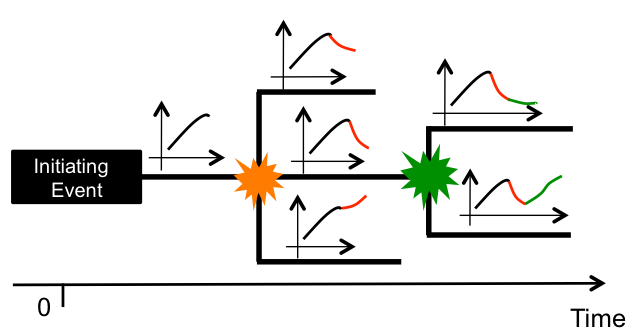
\includegraphics[width=0.8\textwidth]{figures/DET_schemeFlow.png}
  \caption{Dynamic Event Tree Conceptual Scheme.}
   \label{fig:DET_schemeFlow}
\end{figure}
In order to overcome these limitations a ``dynamic'' approach is needed. The DET technique brings several advantages~\cite{ADAPTHakobyan}, among which the fact that it simulates probabilistic system evolution in a way that is consistent with the severe accident model. In DET,  event sequences are run simultaneously starting from a single initiating event. The branchings occur at user specified times and/or when an action is required by the operator and/or the system, creating a deterministic sequence of events based on the time of their occurrence (see Fig.~\ref{fig:DET_schemeFlow}).

This leads to a more realistic and mechanistically consistent analysis of the system taken in consideration. The DPRA, in general, and the DET methodologies, in particular, are designed to take the timing of events explicitly into account which can become very important especially when uncertainties in complex phenomena are considered.

The main idea of this methodology is to let a system code (i.e., RELAP-7) determine the pathway of an accident scenario within a probabilistic ``environment''. \\ Figure~\ref{fig:DET_schemeFlow} schematically shows the DET logic. As already mentioned, the accident sequence starts with an initiating event. Based on an user defined branching logic, driven by \textbf{P}robabilistic \textbf{D}istribution \textbf{F}unctions (PDFs), an event occurs at a certain time instant. The simulation spoons $n$ different branches. In each of them, the branching event determines a different consequence (carrying on associated probabilities). Each sequence continues until another event occurs and a new set of branching is spooned. The simulation ends when an exit condition or a maximum mission time is reached.
%%%%%%%%%%%%%%%%%%%%%%%%%%%%%%
\Section{RAVEN APPROACHING DYNAMIC METHODOLOGIES: ADRAE MODULE}
%%%%%%%%%%%%%%%%%%%%%%%%%%%%%%
\label{sec:DETRavenApproach}
RAVEN is now able to perform DET analysis through the newly developed module "\textbf{A}nalysis of \textbf{D}ynamic \textbf{R}eactor \textbf{A}ccident Evolution" (ADRAE), that has been included in the RAVEN external Python manager.

Following the philosophy of the DET approach, this module lets RELAP-7 find the path of an accident sequence, in a probabilistic point of view. When the system achieves certain conditions that would lead to alternative accident ways (i.e. an event occurs), a sampler generates a new set of branches (new possible scenarios), associating for each a conditional probability.

For the analysis of complex systems, the number of branches may become extremely big. In order to avoid unacceptable growth of problem due by an excessive number of branches, the user needs to specify an exit logic (termination laws), for example maximum mission time, rules based on the simulator physic model (i.e. Maximum temperature of the fuel cladding, etc.), and/or probabilistic thresholds. In other similar codes, one of the most common termination law is a probability cut-off: a branch execution is stopped when its probability falls below a given limit.
%No countermeasures are generally taken to conserve the global probability.

This approach may introduce a big impact on the probability of key events, if the user defined limit is not small enough that the influence on the final branch probability is not negligible.  In order to avoid these issues and preserve the probability conservation, the user can not directly input, in RAVEN, a branching probability cut-off.

As can be inferred from above, RAVEN provides capabilities to:
\vspace{-5mm}
\begin{itemize}
\itemsep0em
\item explore possible pathways through which the system can evolve
\item quantify the probability of these scenarios
\end{itemize}
\vspace{-5mm}
These main tasks are accomplished based on user specified branching and termination laws, model of the system in RELAP-7, probability assignment rules to accident sequences (either by inputed values or/and by distribution functions).
The synergy among the different RAVEN modules gives to the package the flexibility to summarize all the state of art DET capabilities.
Indeed, as in similar tools~\cite{ADAPTHakobyan}, the RAVEN/ADRAE allows the user use different approaches for defying the branching logic:
\vspace{-5mm}
\begin{itemize}
\itemsep0em
\item branching/failures on demand (i.e. time and field triggers)
\item branching based on failure probability distributions
\item multi-branching scenarios
\end{itemize}
\vspace{-5mm}
The list above, in conjunction with the brief overview of the mathematical framework analyzed in section~\ref{sec:mathFramework}, gives an indication on how RAVEN (and the DET module) combines the capabilities present in other similar codes~\cite{ADAPTHakobyan}.

In RAVEN there is no distinction between active (e.g. circulation pumps, valves, controlled systems, etc.) and passive (e.g. steam generators, condensers, pipes, etc.) component behaviors; all are treated as a aleatory uncertainties, since the physical conditions under which a branching would occur for the them are determined by the thermal-hydraulic code RELAP-7 without user ``control''. The user can model also the epistemic uncertainties, uncertainties due by lack of knowledge on the phenomena analyzed (e.g. Heat capacity coefficient, etc.).

In RAVEN, from an user point of view, either the aleatory and epistemic uncertainties are undifferentiated, since the branching laws are inputted in the same way. All triggers are identified by their own PDFs and activated when an user defined probability threshold, on the associated Cumulative Distribution Function (CDF), is overpassed.
The probability thresholds on the CDFs are automatically handled by the DET module; the user only needs to specify them in the input.

The user implements the DET logic in the \verb!Python! control logic input file, under the function named ``\emph{dynamic\_event\_tree}''. In this function, all the features available in RAVEN can be used (online monitoring, controlling, auxiliary system, probability distributions, utilities, etc.).
\begin{figure}[h]
  \centering
     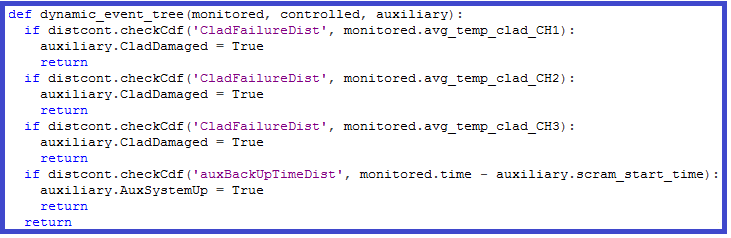
\includegraphics[width=0.8\textwidth]{figures/BranchingLaws.png}
  \caption{Example of DET logic}
   \label{fig:DET_branchLaws}
\end{figure}
\\As an example, Figure~\ref{fig:DET_branchLaws} lists set of branching rules. The ``checkCdf'' function, available in the distribution container, checks if the associated threshold has been passed, and, in case, send a branching signal to RAVEN/RELAP-7 in order to print a restart file, that will be handled by the DET module.
%%%%%%%%%%%%%%%%%%%%%%%%%%%%%%
\Subsection{Software Infrastructure}
\label{sec:CPUInfrastructure}
%%%%%%%%%%%%%%%%%%%%%%%%%%%%%%
In this section the software infrastructure for the DET generation is briefly presented. As already mentioned, the DET module is part of RAVEN \verb!Python! external driver, which represents the core of PRA analysis.
\begin{figure}[h]
  \centering
     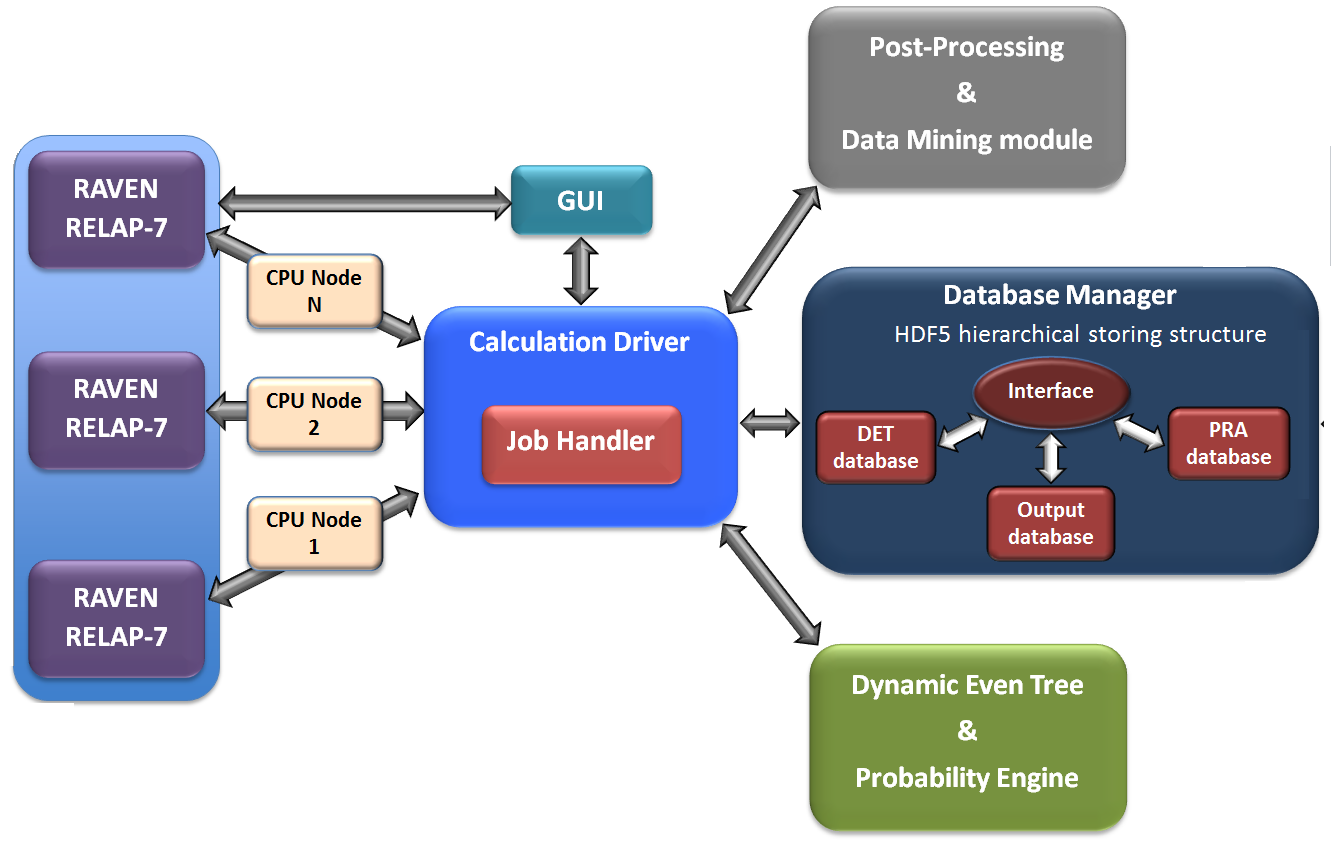
\includegraphics[width=0.75\textwidth]{figures/softwareCalcStructure.png}
  \caption{Software calculation infrastructure scheme}
   \label{fig:softwareInfrastructure}
\end{figure}

The external driver manager has the control of the different modules that support the DET calculation:
\vspace{-5mm}
\begin{itemize}
\itemsep0em
\item General Calculation Driver and Job Handler
\item Visualization and Input supporting GUI
\item DET and Probability Engine
\item Database manager
\item Post-processing and Data Mining module
\item Distribute Computing Environment Interface
\end{itemize}
\vspace{-5mm}
The General Calculation Driver is in charge to communicate information among the different modules. It is the only software branch that is aware of which modules are participating to the calculation.

Figure~\ref{fig:softwareInfrastructure} shows a schematic overview of the calculation structure, highlighting the most important modules that are involved in a DET calculation. Following an initiating event, the DET module provides initiating conditions as well as the duration of the simulation (optionally) to the system simulator (i.e. RAVEN/RELAP-7).
\\The Calculation Driver, through the Job Handler module, runs the simulator until a stopping condition is reached. The DET module decides whether to branch or not depending on the information received, through the general calculation driver, by RAVEN/RELAP-7.
The probability engine is in charge of computing the likelihood of branching generated by trigger signals (e.g. probability threshold on Clad Failure distribution overpassed).  If the DET module decides that $n$ branches are needed, it communicates to the Calculation Driver/Job Handler, that manages the jobs through a queue system, to execute the $n$ branches in $n$ different subprocesses (in parallel, if the machine is multi-processors, in sequence otherwise). The resulting tree structure, branch probabilities, trigger information, and simulation results are sent to the Database manager, that, based on the kind of information received, distributes the data among the sub-structures (DET, PRA, Output databases). The database manager is able to store data in different formats(e.g. HDF5, CSV, etc.).

The user can decide to perform post-processing operations and/or data mining manipulation on the fly, through the Post-processing and data mining module. The whole calculation may be visualized through the RAVEN GUI, that is able to exploit the communication capabilities present in the external calculation driver for following the simulation evolution (e.g. monitored variables or probability evolution through different branches, etc.). \\ The whole calculation infrastructure is designed to be agnostic regarding the machine in which it is running with extremely good performance either in PCs/workstations and HPC clusters.
%%%%%%%%%%%%%%%%%%%%%%%%
\Section{DEMO FOR A PWR PRA ANALYSIS}
\label{sec:demo}
%%%%%%%%%%%%%%%%%%%%%%%%
In order to show the capabilities introduced with the new DET module, a simplified PWR Dynamic PRA analysis is here presented.
\begin{figure}[h]
   \centering
    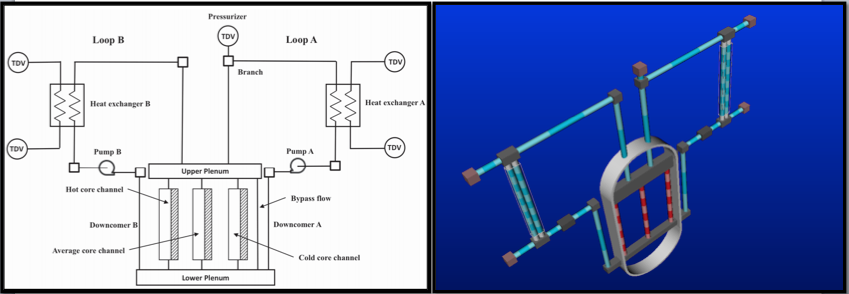
\includegraphics[width=1.0\textwidth]{figures/PWR_TMI_SCHEME.PNG}
    \caption{PWR model scheme}
    \label{fig:PWRmodel}
\end{figure}
Figure~\ref{fig:PWRmodel} shows the scheme of the PWR model. The reactor vessel model consists of the Down-comers, the Lower Plenum, the Reactor Core Model and the Upper Plenum. Core channels (flow channels with heat structure attached to each of them) were used to describe the reactor core. The core model consists of three parallel core channels and one bypass flow channel.
%The hot core channel represents the inner hottest zone of the reactor core. The average core channel represents the mid zone of the core and the cold core channel represents the outer zone of the core, respectively.
There are two primary loops, i.e., loop A and loop B. Each loop consists of the Hot Leg, a Heat Exchanger and its secondary side pipes, the Cold Leg and a primary Pump. A Pressurizer is attached to the Loop A piping system to control the system pressure. A Time Dependent Volume (pressure boundary conditions) component is used to represent the Pressurizer. Since the RELAP-7 code does not have the two-phase flow capability for all needed components yet, single-phase counter-current heat exchanger models are implemented to mimic the function of steam generators in order to transfer heat from the primary to the secondary.

In order to perform a Dynamic PRA analysis on this simplified model, it has been necessary to control unconventional parameters (i.e. inlet/outlet friction factors), since RELAP-7 still has limitations for the component controllable parameters and models. In the following paragraph, the PRA station black out sequence of events is reported.
%%%%%%%%%%%%%%%%%%%%%%%%%%%%%%
\Subsection{Station Black Out (SBO) analysis}
%%%%%%%%%%%%%%%%%%%%%%%%%%%%%%
\label{sec:SBOanalysis}
A PRA analysis has been performed for a Station Black Out accident scenario by sampling the probability thresholds (i.e. branching triggers) on the CDFs of the recovery time of the diesel generators (DGs)  $t_{1}$ (Normal distribution, mu = 1100 s, sigma = 700 s, xMin = 3 s, xMax = $\infty$)  and the clad failure temperature $TC_{f}$  (Triangular distribution, xPeak = 1477.59\footnote{Typical PRA success criteria.} K, xMin~ =~1255.37\footnote{10 CFR50.46 limit.} K, xMax = 1699.82 K~\cite{Urbanic1978}).

Two sets of DET calculations have been run:
\vspace{-5mm}
\begin{itemize}
    \item ESBP: equally spaced branching probability thresholds
    \item ESVV: branching probability thresholds corresponding to equally spaced variable values ($TC{f}$ and $t_{1}$)
\end{itemize}
\vspace{-5mm}
The probability threshold values for both DET calculations are reported below:
\vspace{-5mm}
 \begin{itemize}
   \item \textbf{First DET calculation (ESPB)} :
   \begin{itemize}
       \item DGs recovery time distribution (Fig.~\ref{fig:DGrecTime} - green points):
       \begin{itemize}
            \item Probability Thresholds: 0.1, 0.2, 0.3, 0.4, 0.5, 0.6, 0.7, 0.8, 0.9
            \item Variable Values           : 382.52, 621.06, 813.45, 985.89, 1151.28, 1319.82, 1502.67, 1718.86, 2021.09
       \end{itemize}
       \item Clad Failure Temperature distribution (Fig.~\ref{fig:CladFailureDist} - green points):
       \begin{itemize}
            \item Probability Thresholds: 0.1, 0.2, 0.3, 0.4, 0.5, 0.6, 0.7, 0.8, 0.9
            \item Variable Values           : 1354.75, 1395.92 , 1427.50, 1454.13, 1477.59, 1501.05, 1527.68, 1559.27, 1600.43
       \end{itemize}
    \end{itemize}
   \item \textbf{Second DET calculation (ESVV)}:
   \begin{itemize}
       \item DGs recovery time distribution (Fig.~\ref{fig:DGrecTime} - red points):
       \begin{itemize}
            \item Probability Thresholds: 0.0433, 0.1901, 0.4086, 0.6451, 0.8315, 0.9383, 0.9829
            \item Variable Values           : 200.00, 600.00, 1000.00, 1400.00, 1800.00, 2200.00, 2600.00
       \end{itemize}
       \item Clad Failure Temperature distribution (Fig.~\ref{fig:CladFailureDist} - red points):
       \begin{itemize}
            \item Probability Thresholds: 0.0200, 0.0910, 0.2120, 0.3840, 0.5960, 0.7730, 0.8990, 0.9750
            \item Variable Values           : 1300.00, 1350.00, 1400.00, 1450.00, 1500.00, 1550.00, 1600.00, 1650.00
       \end{itemize}
    \end{itemize}
\end{itemize}
\vspace{-5mm}

\begin{figure}
 \begin{minipage}[b]{8.5cm}
   \centering
   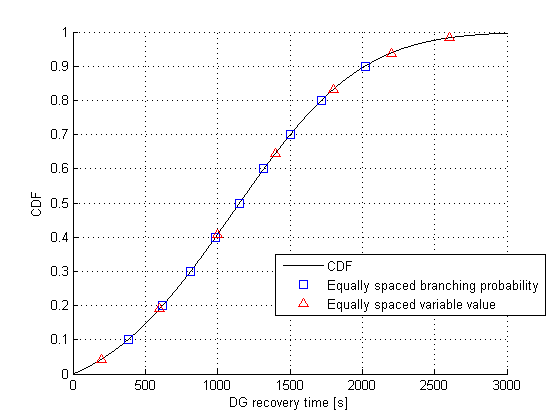
\includegraphics[width=9cm]{figures/DieselRecTime.png}
   \caption{Diesel Generator Recovery Time CDF.}
   \label{fig:DGrecTime}
 \end{minipage}
 \ \hspace{2mm} \hspace{3mm} \
 \begin{minipage}[b]{8.5cm}
  \centering
   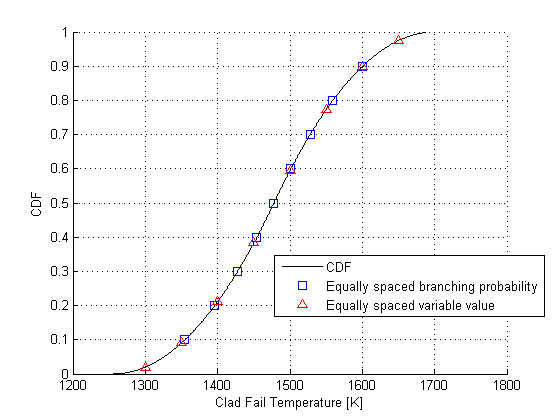
\includegraphics[width=9cm]{figures/CladFailure.png}
   \caption{Clad Failure Temperature CDF.}
   \label{fig:CladFailureDist}
 \end{minipage}
\end{figure}
In addition, a Monte-Carlo (MC) calculation has been run. It has been decided to perform only 50 samplings (randomly sampling $t_{1}$ and $TC_{f}$), in order to maintain a similar number of ``samples''  among MC and DET calculations.

The SBO transient is based on the following sequence of events (starting from a steady-state operational condition of a Nuclear Power Plant~\cite{relap7FY12}):
\vspace{-5mm}
 \begin{itemize}
   \item 100.0 seconds: transient begins
   \item 101.0 seconds: loss of power grid and immediate shutdown of the reactor(scram):
   \begin{itemize}
       \item Pump coast-down;
       \item Decay heat power;
       \item Diesel Generators and residual heat removal system (RHRS) not available.
    \end{itemize}
   \item $t_{1}$: recovery of the diesel generators
   \item $t_{2}$: end of transient either for clad failure or 3000 seconds of simulation (PRA success)
\end{itemize}
\vspace{-5mm}
Since the scope of this demo is to show the new capabilities contained in RAVEN, and RELAP-7 is not optimized for long simulation times, the transient has been accelerated in order to simulate a maximum of 3000 seconds.
In the following section, the simulations results are shown and discussed.
%%%%%%%%%%%%%%%%%%%%%%%%%%%%%%
\Subsection{Results}
%%%%%%%%%%%%%%%%%%%%%%%%%%%%%%
DET analyses have been performed, obtaining the following data sets:
\vspace{-5mm}
\begin{itemize}
\item \emph{ESBP DET I}: 37 DET branches resulting in 18 complete histories
\item \emph{ESVV DET II}: 31 DET branches resulting in 15 complete histories
\end{itemize}
\vspace{-5mm}
Note that the number of branches (and, hence, the number of histories) are different between the two different calculation performed since a difference number of branching thresholds have been considered (see Section~\ref{sec:SBOanalysis}).

\begin{figure}
 \begin{minipage}[b]{8.5cm}
   \centering
   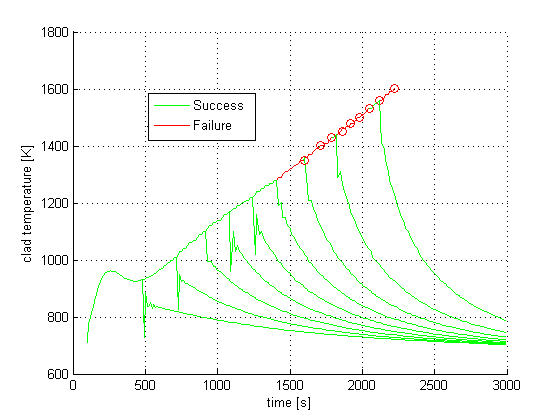
\includegraphics[width=9cm]{figures/DETpbClad.png}
   %\caption{Clad Temperature evolution in hot core channel (case ESBP DET I).}
   %\label{fig:DETpbClad}
 \end{minipage}
 \ \hspace{2mm} \hspace{3mm} \
 \begin{minipage}[b]{8.5cm}
   \centering
   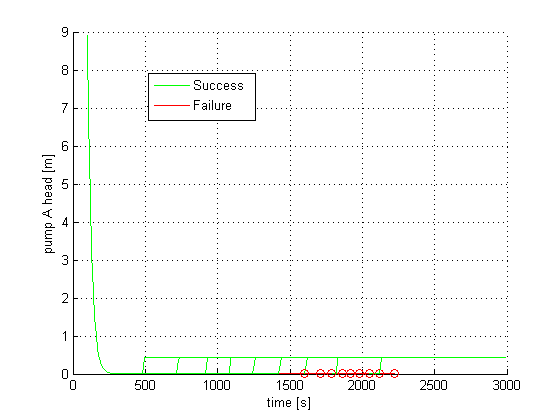
\includegraphics[width=9cm]{figures/DETpbHead.png}
   %\caption{Pump Head evolution (case ESBP DET I).}
   %\label{fig:DETpbHead}
 \end{minipage}
\caption{Case ESBP DET I: Clad Temperature and Pump Head temporal profiles (all histories)}
\label{fig:ESBPall}
\end{figure}
\vspace{-5mm}

Figures~\ref{fig:ESBPall} and~\ref{fig:ESVVall} show the histories obtained for the ESBP DET I and ESVV DET II respectively.
Following the station back-out condition, the pump head decreases (pump coast-down) and the temperature of the core rises since reactor core cooling is not available. Such temperature increasing continues until one of the following conditions occurs:
\vspace{-5mm}
\begin{itemize}
\item temperature of the clad reaches the clad failure temperature, indicated with a red circle (red scenarios in Fig.s~\ref{fig:ESBPall} and~\ref{fig:ESVVall}), or,
\item DG power is restored (green scenarios in Fig.s~\ref{fig:ESBPall} and~\ref{fig:ESVVall}).
\end{itemize}
\vspace{-5mm}
Note that following the recovery of the DG power (green scenarios) the clad temperature drops  and an oscillating behavior can be observed.
This is caused by the sudden activation of the auxiliary core cooling system.

From a safety point of view, the most important information is the frequency of failures in the phase space. This information can be shown plotting the final outcome (green points for system success and red points for system failure) of all the simulations for each data sets in a $2$-dimensional space (DG recovery time vs. clad failure temperature) as shown in Fig.~\ref{fig:DET_LS}.
The limit surface, i.e. the boundary between system failure and system success regions (black line), is also indicated in Fig.~\ref{fig:DET_LS}. Such boundary was determined using a Support Vector Machine (SVM) based algorithm~\cite{mandelliSVMANS}.
Note that most of the points in this $2$-dimensional space (for both data sets) lie in proximity  of the limit surface while samples generated by a classical Monte-Carlo based algorithm would be evenly distributed (see Fig.~\ref{fig:MonteCarloLS}).
This example shows one of the advantages of DET algorithm in terms of ``choosing'' the best set of candidate samples when performing PRA analyses.

%%%%%%%%%%

\begin{figure}
 \begin{minipage}[b]{8.5cm}
  \centering
   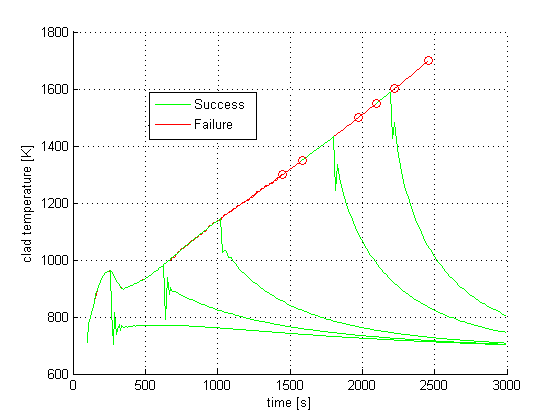
\includegraphics[width=9cm]{figures/DETvarClad.png}
   %\caption{Clad Temperature evolution in hot core channel (case ESVV DET II).}
   %\label{fig:DETvarClad}
 \end{minipage}
 \ \hspace{2mm} \hspace{3mm} \
 \begin{minipage}[b]{8.5cm}
  \centering
   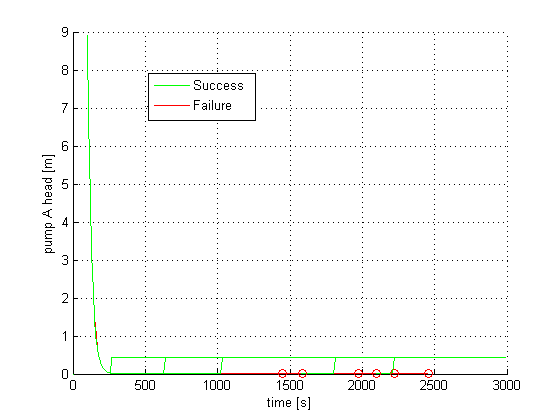
\includegraphics[width=9cm]{figures/DETvarHead.png}
   %\caption{Pump Head evolution (case ESVV DET II).}
   %\label{fig:DETvarHead}
 \end{minipage}
\caption{Case ESVV DET II: Clad Temperature and Pump Head temporal profiles (all histories)}
\label{fig:ESVVall}
\end{figure}

%%%%%%%%%%%%%%%%%
\begin{figure}
 \begin{minipage}[b]{8.5cm}
   \centering
   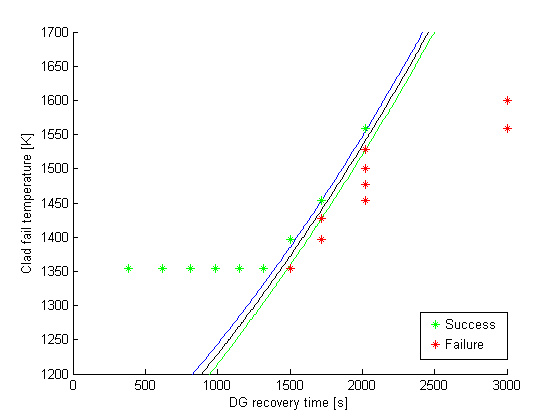
\includegraphics[width=9cm]{figures/DET_LS_pb.png}
   %\caption{Limit Surface (case ESBP DET I).}
   %\label{fig:DETvarLS}
 \end{minipage}
 \ \hspace{2mm} \hspace{3mm} \
 \begin{minipage}[b]{8.5cm}
  \centering
   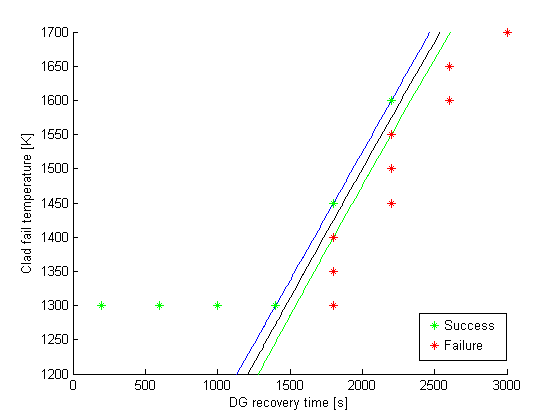
\includegraphics[width=9cm]{figures/DET_LS_var.png}
   %\caption{Limit Surface (case ESVV DET II).}
   %\label{fig:DETpbLS}
 \end{minipage}
\caption{DET Limit Surface: case ESBP DET I(left) and case  ESVV DET II (right)}
\label{fig:DET_LS}
\end{figure}
\begin{figure}[h]
   \centering
    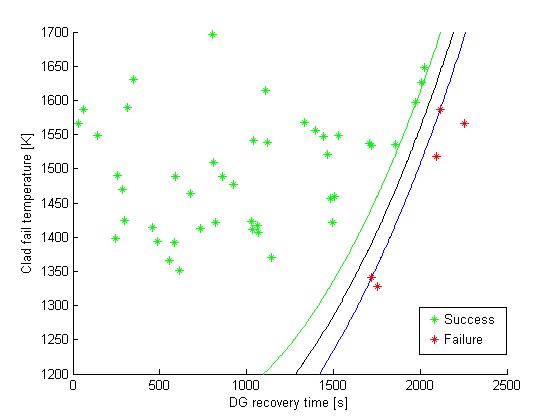
\includegraphics[width=0.6\textwidth]{figures/MC.png}
    \caption{Monte-Carlo Limit Surface.}
    \label{fig:MonteCarloLS}
\end{figure}

%Figure~\ref{fig:distributionResults} shows the distribution of the maximum temperature reached by the clad in the core channels (blue histogram) and compares it with the distribution of clad failure temperature (red histogram).
%Although there is large overlapping of the two distributions, which indicates a high failure probability of the system considered, the scope of the analysis was just to show  RAVEN capabilities to perform stochastic analysis of relatively complex systems.
%The distribution of the clad temperature already accounts for the simulations that have been stopped for having reached the corresponding failure temperature. Therefore, the overlapping of the two distributions is not representative of the total failure rate. Instead, the total failure rate could be inferred from the steep decrease on the higher temperature side of the number of counts with respect the lower temperature one. The probability of failure is artificially elevated with respect a real case in order to keep the effort bounded while illustrating the full RAVEN capabilities.
%%%%%%%%%%%%%%%%%
\section{CONCLUSIONS AND FUTURE WORK}
%%%%%%%%%%%%%%%%%
This paper presented RAVEN as a tool to perform dynamic PRA through Dynamic Event Tree sampling. In particular, the software structure and all the components that are involved in the computation have been described, including system simulator (i.e., RELAP-7) and the control logic, characterized by monitor system dynamics and on-line control of selected parameters.
An example of PRA analysis has been also shown for a SBO scenario for a simplified PWR loop.
The description of the implementation for such case demonstrates how the flexibility of the software framework provides state-of-the-art tools to perform Dynamic PRA, uncertainty quantification and plant control.
Next capabilities, to be implemented to RAVEN, and currently under development, include adaptive dynamic event tree generation, adaptive sampling~\cite{mandelliSVMANS} and advanced data mining algorithms~\cite{mandelliEsrel2011,MandelliClusteringRESS}.
%%%%%%%%%%%%%%%%%%%%%%%%%%%%%%%%%%%%%%%%%%%%%%%%%%%%%%%%%%%%%%%%%%%%%%%%%%%%%%%%
\section*{ACKNOWLEDGMENT}
%%%%%%%%%%%%%%%%%%%%%%%%%%%%%%%%%%%%%%%%%%%%%%%%%%%%%%%%%%%%%%%%%%%%%%%%%%%%%%%%
This work is supported by the U.S. Department of Energy, under DOE Idaho Operations Office Contract DE-AC07-05ID14517. Accordingly, the U.S. Government retains a nonexclusive, royalty-free license to publish or reproduce the published form of this contribution, or allow others to do so, for U.S. Government purposes.

\bibliographystyle{ieeetr}
\bibliography{bibl}


\end{document}


